\chapter{A rendelések adatainak nyilvántartása}

%Itt magáról az adatmodellről van szó gyakorlatilag. Itt érdemes kifejteni, hogy milyen adat, és hol kerül majd tárolásra. Az ER jellegű diagram, illetve az SQLAlchemy-s modellek egyszerűsített változata kellene majd ide.

%A rendelések adatainak nyilvántartása
Az adatbázis tervezése során az egyik fő célom az volt, hogy könnyen módosítható, illetve kibővíthető legyen a rendszer. Első lépésként a fontosabb egyedeket határoztam meg, majd a köztük lévő kapcsolatokat. A dolgozatom készítése során elkészítettem két kezdetleges adatmodellt, amelyeknek az összefésüléséből megszületett a végleges adatmodell. Az alkalmazás implementálása során számos alkalommal kellett módosítanom az adatbázist.

Az általam tervezett adatmodell egyes táblái és a köztük lévő kapcsolatok \aref{fig:rendeles_sema} ábrán láthatók.

\begin{figure}
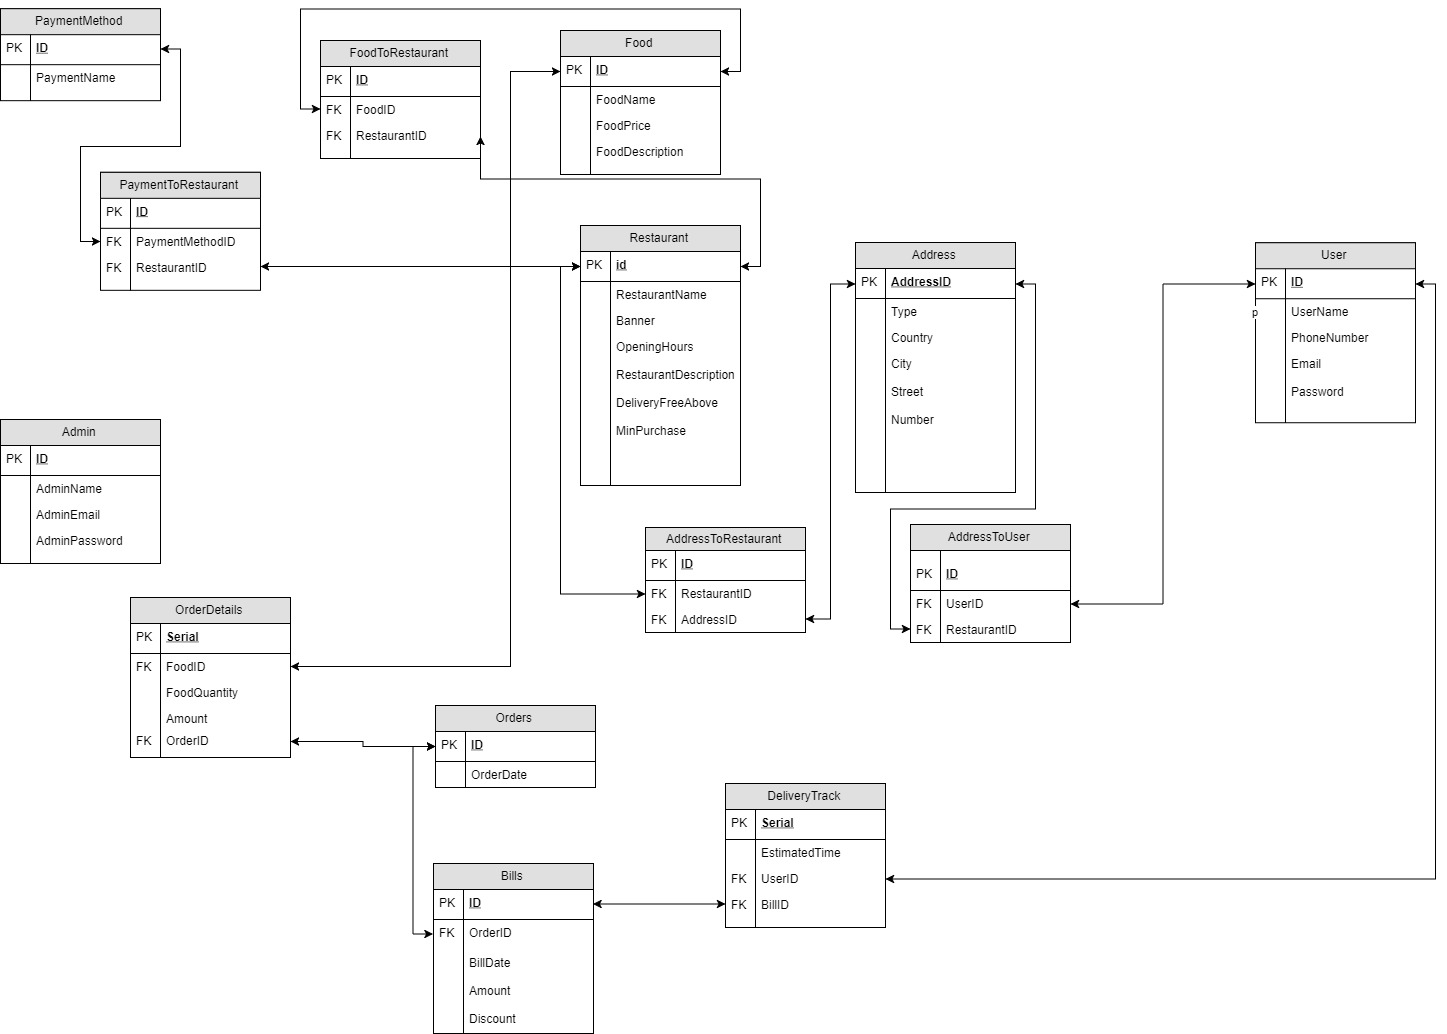
\includegraphics[scale=0.3]{kepek/rendeles_sema.jpg}
\caption{A rendelések adatait kezelő adatábis sémája}
\label{fig:rendeles_sema}
\end{figure}

\section{users}

Az online alkalmazásomon keresztül való étel rendeléshez regisztrált felhasználónak kell lenni. Ez a tábla a regisztrált felhasználókról tartalmaz információkat, illetve az adatbázisban lévő éttermek tulajdonosairól. Minden felhasználó rendelkezik egy azonosítóval, egy kereszt egy vezeték és egy felhasználónévvel, jelszóval továbbá egy telefonszámmal, egy email címmel. Mindegyikhez tartozik egy address, illetve abban az esetben a felhasználó típusa 1-es, - tehát étterem tulajdonos - akkor tartozik hozzá egy restaurant.

\begin{tabular}{|p{3cm}|p{10cm}|}
\hline
user\_id & Elsődleges kulcs, a felhasználó azonosítója. \\
\hline
first\_name & A regisztrált felhasználó keresztneve. \\
\hline
last\_name & A regisztrált felhasználó vezetékneve. \\
\hline
user\_name & A regisztrált felhasználó felhasználóneve. \\
\hline
password & A felhasználó jelszava. \\
\hline
phone\_number & A felhasználó telefonszáma. \\
\hline
email & A felhasználó email címe. \\
\hline
user\_role & Felhasználó típus, lehetséges értékek: 0: egyszerű felhasználó 1: étterem tulajdonos \\
\hline
\end{tabular}

\section{restaurants}

Ez a tábla tartalmazza az éttermeket és a hozzájuk tartozó információkat. A tábla minden bejegyzéséhez tartozik egy address, illetve minden étteremhez tartozik egy user is. Egy étteremhez tartozik egy azonosító, egy név, egy leírás étteremről, meg kell adni az étteremből való rendelés minimális összegét továbbá a kiszállítás maximális időtartamát. Opcionálisan tartalmazhatja a kiszállítás árát, a kiszállítás minimális idejét illetve az étterem logójának URL címét.
Kötelező mezők

\begin{tabular}{|p{3cm}|p{10cm}|}
    \hline
    restaurant\_id & Elsődleges kulcs, az étterem azonosítója. \\
    \hline
    restaurant\_name & Az étterem neve. \\
    \hline
    restaurant\_description & Az étterem leírása. \\
    \hline
    min\_order & Az étteremből való rendelés minimális összege. \\
    \hline
    delivery\_max\_time & Az étteremből való kiszállítás maximális időtartama. \\
    \hline
\end{tabular}

\section{meals}

Ebben a táblában tárolom az adott éttermek által forgalmazott ételeket, italokat. A táblának egy bejegyzése egy étteremhez tartozik, de egy adott étteremhez több meal is tartozhat. A táblában minden bejegyzéshez tartozik egy azonosító, egy név, egy leírás, a termék ára, a terméket forgalmazó étterem azonosítója illetve opcionálisan meg lehet adni a termék logójának URL címét.
Kötelező mezők

\begin{tabular}{|p{3cm}|p{10cm}|}
    \hline
    meal\_id & Elsődleges kulcs, a termék azonosítója \\
    \hline
    meal\_name & Az étel neve. \\
    \hline
    meal\_description & Az étel leírása \\
    \hline
    meal\_price & Az étel ára. \\
    \hline
    restaurant\_id & Idegen kulcs, a terméket forgalmazó étterem azonosítója. \\
    \hline
\end{tabular}

\section{addresses}

Az addresses tábla tartalmazza a felhasználók és az éttermek címéhez tartozó információkat. Mindegyik vagy egy étteremhez vagy egy felhasználóhoz tartozik, egy felhasználóhoz több cím is tartozhat. Egy címhez mindig tartozik egy azonosító, egy típus(szállítási, vagy lakcím), egy város, utca illetve házszám, továbbá vagy egy étterem vagy egy felhasználó azonosító attól függően, hogy étteremhez vagy felhasználóhoz tartozik e a cím.
Kötelező mezők

\begin{tabular}{|p{3cm}|p{10cm}|}
    \hline
    address\_id & Elsődleges kulcs, a cím azonosítója. \\
    \hline
    address\_type & A cím típusa, értéke lehet: 0: lakcím 1: szállítási cím \\
    \hline
    address\_city & A cím város komponense. \\
    \hline
    address\_street & A cím utca komponense. \\
    \hline
    address\_number & A cím házszám komponense. \\
    \hline
    restaurant\_id & Idegen kulcs, a címhez tartozó étterem azonosítója \\
    \hline
    user\_id & Idegen kulcs, a címhez tartozó felhasználó azonosítója \\
    \hline
\end{tabular}

\section{orders}

Ez a tábla tartalmazza a rendeléseket. Egy rendeléshez order\_meal-ek tartoznak, ezek tartalmazzák a megrendelt termékek adatait. Minden rendelés tartalmaz egy azonosítót, egy dátumot, egy árat, illetve a rendelést leadó felhasználó azonosítóját.
Kötelező mezők

\begin{tabular}{|p{3cm}|p{10cm}|}
\hline
order\_id & Elsődleges kulcs, a rendelés azonosítója. \\
\hline
order\_date & A rendelés dátuma. \\
\hline
order\_price & A rendelés összege. \\
\hline
user\_id & A rendelést leadó felhasználó azonosítója \\
\hline
\end{tabular}

\section{order\_meals}

Ez a tábla a felhasználó által kosárba helyezett termékekről tartalmaz információkat. Egy order\_meal bejegyzés egy megrendelt termékről tárol adatokat. Minden bejegyzés tartalmaz rendelés azonosítót, ami megadja, hogy egy order\_meal melyik rendeléshez tartozik. Egy rendeléshez több order\_meal is tartozhat. Mindegyeik order\_meal-hez tartozik az rendelés azonosítón kívül egy azonosító, egy darabszám, egy ár, illetve egy termék azonosító.
Kötelező mezők

\begin{tabular}{|p{3cm}|p{10cm}|}
    order\_meals\_id & Elsődleges kulcs, az order\_meal azonosítója. \\
    \hline
    order\_meals\_quantity & A megrendelt termék darabszáma. \\
    \hline
    order\_meals\_price & A megrendelt termék ára. \\
    \hline
    order\_id & Idegen kulcs, a rendelés azonosítója, amihez az order\_meal tartozik. \\
    \hline
    meal\_id & Idegen kulcs, az order\_meal-hez tartozó termék azonosítója. \\
    \hline
\end{tabular}

\section{payments}

Ebben a táblában az éttermek által biztosított fizetési lehetőségeket tárolom. Minden bejegyzéséhez tartozik egy étterem azonosító, amivel meg lehet adni, hogy az adott fizetési lehetőségek melyik étteremhez tartoznak. Egy ilyen bejegyzés tartalmazza az imént említett étterem azonosítót, továbbá egy azonosítót, és különböző fizetési lehetőségeket, melyeknek az értéke 0, ha az adott étteremnél nem lehet ilyen módon fizetni, illetve 1 ha lehet.

\begin{tabular}{|p{3cm}|p{10cm}|}
    payment\_id & Elsődleges kulcs, a payment azonosítója. \\
    \hline
    cash & Készpénzes fizetési lehetőség. \\
    \hline
    creditcard & Bankkártyás fizetési lehetőség. \\
    \hline
    szep\_card & SZÉP kártyás fizetési lehetőség. \\
    \hline
    erzsebet\_voucher & Erzsébet utalvány elfogadása. \\
    \hline
    restaurant\_id & Idegen kulcs, az étterem azonosítója, amelyikhez tartozik az adott payment. \\
    \hline
\end{tabular}

\section{Back-End}

A szerver oldalon egy többrétegű struktúrát hoztam létre. Ebben a fejezetben a két felső réteget, a Flask alkalmazást és a nyilvántartó csomagot fogom részletezni

\subsection{Nyilvántartó csomag}

A nyilvántartó csomagban lévő metódusok végzik a lekérdezéseket, ezeket a metódusokat hívom meg a flaskos rétegben. A nyilvántartó csomag egy absztrakciós szintet biztosít, elfedi az alsóbb rétegek technikai részleteit. A közbenső réteg bevezetésének számos előnye volt. Rövidebb és átláthatóbb lett a Flask fájl, mivel a lekérdezések, ellenőrzések és eredmények feldolgozására átkerült a nyilvántartó csomag függvényeibe. Így a Flask szinte csak a paraméterek lekérdezésével és a válaszok előállításával foglalkozik.

A nyilvántartó csomag egyik legnagyobb előnye a későbbi továbbfejlesztési lehetőségekben rejlik. Ha a későbbiekben szeretnék egy mobil vagy asztali alkalmazást csinálni, csupán a Flaskos réteget kellene lecserélni, a back-end többi része maradhatna.

A nyilvántartó library 6 pyton fájlt tartalmaz, melyekben különböző függvények lettek implementálva. A további ezeket a fájlokat és függvényeket fogom ismertetni.

\subsection{\texttt{Adddress.py}}

\begin{itemize}
    \item \texttt{query\_cities()}: Az adatbázisban található éttermekhez rendelt címeket kérdezi le. Dictionary-k listájaként a címek város komponensét adja vissza.
\end{itemize}

\subsection{\texttt{Meal.py}}

\begin{itemize}
    \item \texttt{query\_meals(restaurant\_id)}:
        Az adatbázisból a paraméterként megadott azonosítójú étterem kínálatában lévő ételeket kérdezi le, az eredmény dictionary-k listájaként adja vissza.
    \item \texttt{query\_meal\_types(restaurant\_id)}:
        A paraméterként kapott étterem kínálatában lévő ételek típusait kérdezi le az adatbázisból, az eredményt ez a függvény is dictionary-k listájaként adja vissza.
    \item \texttt{add\_new\_meal(newMeal)}:
        A paraméterként kapott adatokból létrehoz egy új Meal objektumot, és azt menti az adatbázisban.
    \item \texttt{remove\_meal(removable\_meal)}:
        Az adatbázisból lekérdezi a paraméterként kapott Meal objektum azonosítójával megegyező azonosítójú ételt, és azt törli az adatbázisból. Törlés után véglegesíti az adatbázis módosításokat.
    \item \texttt{query\_meal\_data\_by\_id(meal\_id)}:
        Paraméterként kap egy étel azonosítót. Lekérdezi az adatbázisból a kapott azonosítóval megegyező azonosítójú ételt, a kapott eredményt a függvény dictinary-ként adja vissza.
    \item \texttt{edit\_meal(params)}:
        Ez a függvény kerül meghívásra, amikor egy adatbázisban lévő étel adatait akarjuk módosítani. Paraméterként kap egy étel azonosítót, egy étterem azonosítót, és a módosítandó adatokat. A kapott étel azonosítóval megegyező azonosítójú ételt lekérdezi az adatbázisból, az adatmódosításokat elvégzi, és véglegesíti az adatbázis módosítást. A status nevű változóval tér vissza, melynek értéke sikeres módosítása esetén 200, sikertelen esetén 401.
    \item \texttt{query\_meal\_type\_stat(username, restaurant\_id)}:
        A paraméterként kapott felhasználónévvel megegyező felhasználónevű user-t lekérdezi az adatbázisból. A Meal táblából lekérdezi azokat az ételeket étel típus szerint csoportosítva, amiknek az étterem azonosítójuk megegyezik a paraméterként kapott azonosítóval. Az Order adatbázis táblából lekérdezi azokat a rendeléseket, melyeknél az étterem azonosító megegyezik a kapott azonosítóval. A lekérdezések eredményének segítségével összeszámolja, hogy a paraméterként kapott azonosítóval rendelkező étteremben leadott rendelésekben hány darab van a különböző ételtípusokból. Az eredményt a függvény dictionary-k listájaként adja vissza.
\end{itemize}

\subsection{\texttt{Order.py}}

\begin{itemize}
\item \texttt{checkout\_order(newOrder)}:
Lekérdezi az adatbázisból a paraméterként kapott azonosítójú ételt, és a kapott felhasználónévvel megegyező felhasználónevű usert. Létrehoz egy új rendelés objektumot a paraméterként kapott, és a lekérdezett értékekből. Az adatbázis mentése előtt módosítja a felhasználó jutalompontjainak a számát egy képlet alapján. A függvény még létrehoz egy Order\_meals objektumot is a paraméterként kapott adatokból. Ezeket az adatbázis műveleteket is véglegesíti. Amennyibben minden sikeres volt a függvény visszatér a status változóval, melynek 200-ra állítja be az értékét.
\item \texttt{query\_orders()}:
Lekérdezi az adatbázisban található összes rendelést, az eredményt dictionary-k listájaként adja vissza.
\item \texttt{query\_my\_orders(username, restaurant\_id)}:
Az adatbázisból lekérdezi a paraméterként kapott felhasználónévvel megegyező nevű felhasználót, és a kapott étterem azonosítóval egyező azonosítójú éttermet. Továbbá lekérdezi az Order táblából azokat a rendeléseket, melyeknek az étterem azonosítója megegyezik a kapott azonosítóval. A lekérdezések eredményéből összeállít egy listát, amiben dictionary-k vannak tárolva, és ezt adja vissza eredményként.
\end{itemize}

\subsection{\texttt{Payment.py}}

\begin{itemize}
\item \texttt{query\_payments(restaurant\_id)}:
Lekérdezi az adatbázisból azokat a fizetési módokat, melyeknek az étterem azonosítójuk megegyezik a paraméterként kapottal. A kapott eredményen végig iterál egy for ciklussal, amelyik fizetési mód értéke 1, ahhoz hozzá rendeli a Payment nevű enum osztályból a megfelelő értéket. A függvény egy listával tér vissza, amiben dictionary-k vannak.
\item \texttt{query\_payment\_type\_stat(username, restaurant\_id)}: 
A paraméterként kapott felhasználónévvel megegyező felhasználónevű user-t lekérdezi az adatbázisból. A PaymentTable táblából azt a bejegyzést, amelyiknek az étterem azonosítója megegyezik a paraméterben kapottal. A függvény összeszámolja, hogy az adott étteremben leadott rendelések során milyen gyakorisággal választották az egyes fizetési módokat. Az eredményt dictionary-k listájaként adja vissza.
\end{itemize}

\subsection{\texttt{Restaurant.py}}

\begin{itemize}
\item \texttt{query\_restaurants()}:
Az adatbázisban lévő összes éttermet lekérdezi, az eredményt dictionary-k listájaként adja vissza.
\item \texttt{query\_my\_restaurants(current\_username)}:
A paraméterként kapott felhasználónévvel megegyező felhasználónevű usert lekérdezi a User táblából. Restaurant táblából lekérdezi azokat az éttermeket, melyek felhasználó azonosítója megegyezik a lekérdezed felhasználó azonosítójával. Az eredmény dictionary-k listájában adja vissza.
\item \texttt{query\_restaurant\_by\_name(newRestaurant)}:
A függvény az adatbázisból lekérdezi a paraméterben kapott névvel megegyező nevű éttermet, és azt adja vissza eredményként.
\item \texttt{add\_new\_restaurant(newRestaurant)}:
A paraméterként kapott felhasználónévvel megegyező nevű felhasználót lekérdezi. Létre hozz egy új étterem objektumot a paraméterben kapott, és a lekérdezett adatokból. Felviszi az új éttermet az adatbázisba, és véglegesíti az adatbázismódosításokat. Egy új cím objektumot is létrehoz, szintén a paraméter adatokból, és felviszi az adatbázisba. Az új cím objektumhoz hozzárendeli az új étterem azonosítóját.
\item \texttt{query\_restaurant\_by\_id(params)}:
A paraméterként megadott azonosítójú éttermet adja vissza.
\item \texttt{edit\_restaurant(params, restaurant)}:
Lekérdezi azt a felhasználót, amelyikhez hozzá van rendelve a paraméterként kapott azonosítójú étterem. Ellenőrzi, hogy a paraméterben kapott jelszó megegyezik e lekérdezett felhasználó jelszavával, ha igen akkor elvégzi a módosításokat, menti az adatbázist, a status változott 200-ra állítja, és visszatér vele. Amennyiben a két jelszó nem egyezik, a status változó értéke 401 lesz, és azzal tér vissza.
\item \texttt{query\_my\_restaurant\_data(restaurant\_id)}:
Az adatbázisból lekérdezi a paraméterként kapott azonosítójú éttermet, és a hozzárendelt címet. Az adatokat egy dictionary-ben adja vissza.
\end{itemize}

\subsection{\texttt{User.py}}

\begin{itemize}
    \item \texttt{query\_user\_by\_name(newUser)}:
A paraméterként kapott felhasználónevű felhasználót lekérdezi, és visszatér vele.
\item \texttt{user\_registration(newUser)}:
A paraméterként kapott adatokból létrehoz egy új User objektumot, és menti az adatbázisban. Egy Address objektumut is létrehoz a kapott adatokból, és hozzá rendeli a létrehozott felhasználót. 
\item \texttt{query\_users()}:
Az adatbázisban lévő összes felhasználót lekérdezi, és egy dictionary-ket tartalmazó listában adja vissza őket.
\item \texttt{edit\_user(params)}:
A paraméterként kapott felhasználónevű felhasználót lekérdezi, majd ellenőrzi, hogy a paraméterként kapott jelszó egyezik e a lekérdezett felhasználó jelszavával. Ha egyezik módosítja a felhasználó jelszavát, menti az adatbázist, status változót 200-ra állítja és visszatér vele. Amennyiben nem egyezik a status változót 401-re állítja, és visszatér vele.
\item \texttt{query\_user\_data(username)}:
A paraméterként kapott felhasználónevű felhasználót lekérdezi, majd a hozzá tartozó címeket is. A kapott eredményeket dictionary-k listájában adja vissza.
\item \texttt{user\_login(current\_user)}:
Lekérdezi az adatbázisban található összes felhasználót, majd egy for ciklussal végig iterál a kapott eredményen. A ciklus magban vizsgálja, hogy a paraméterként kapott felhasználónévvel talál e megegyezőt, ha igen, akkor megvizsgálja a szintén paraméterként kapott jelszó helyességét is. Deklarál egy payload dictionary-t a felhasználónévből, azonosítóból és egy generált számsorból. A JWT encode függvényének meghívásával létrehoz egy tokent, az encode paraméterként megkapja a payload-ot és egy titkos kulcsot. Az autentikációhoz szükséges adatokat a login\_user dictionary-ban tárolja, és sikeres azonosítás esetén ezzel tér vissza. Sikertelen bejelentkezés esetén a status változó értékét 202-re állítja és azzal tér vissza.
\end{itemize}

\section{Flask webalkalmazás}

A klienstől érkező kérések feldolgozására az alkalmazás a Flask webes mikro keretrendszert használja. A flaskos réteg http válaszokat küld a kliensnek, melyeben az adatok JSON formátumúak. A flaskos réteg és az alsóbb rétegek között van egy közbenső réteg, az általam készített nyilvántartó csomag. A nyilvántartó csomagban lévő metódusok végzik a lekérdezéseket, ezeket a metódusokat hívom meg a flaskos rétegben. A közbenső réteg bevezetésére a későbbi továbbfejlesztési lehetőségek miatt volt szükség. A flask és a nyilvántartó csomag bemutatására a hetedik fejezben fog sor kerülni.

A flaskos réteg a kliens oldalról érkező kérések feldolgozását végzi. Amennyiben a kapott kérésben volt paraméter, megvizsgálja annak helyeségét. A válaszhoz szükséges adatok előállítását a nyilántartó csomag végzi, a flaskos rétegben csak meg kell hívni a megfelelő metódusokat a szükséges paraméterezéssel. Az előállított adatokból létrehozza a választ, és JSON formátumban továbbítja a kliensnek.

\subsection{\texttt{Index.py}}

Az index.py fájlban van implementálva a flaskos réteg. Minden flaskos függvény a route() dekorátorral van ellátva, ez a dekorátor azt írja le, hogy melyik URL-re hivatkozza fog meghívódni az adott függvény.

A továbbiakban az útvonalakat és a hozzájuk tartozó \textit{endpoint} függvényeket fogom részletezni.
A függvények neve és URL címek (\textit{az index függvény kivételével}) megegyeznek, ezért az alpontok címénék mindig az adott függvény URL-jét fogom megadni.

\begin{itemize}
\item \texttt{/}:
Az index() függvény meghívása a „/” URL-re hivatkozva történik. Ez az alkalmazás megnyitásakor és főoldal gombra való kattintáskor fordul elő, ilyenkor elküldi az index.html fájlt.
\item \texttt{/registration}:
Új felhasználót visz fel az adatbázisba. Először lekérdezi a paraméterben kapott felhasználónevű usert, megvizsgálja, hogy foglalt e már ez a felhasználónév. A lekérdezéshez a query\_user\_by\_name() függvényt használja a newUser paraméterrel, melyben a regisztrálni kívánt felhasználó adatai vannak. Ha foglalt a felhasználónév, akkor a 409-es hibakóddal tér vissza. Ha nem foglalt, meghívja a user\_registration() függvényt szintén a newUser paraméterrel, a függvény elvégzi a szükséges adatbázisműveleteket, majd visszatér a registration() metódushoz, ami 200-as státuszkódot küld válaszként a kliens oldalra.
\item \texttt{/checkout}:
Ez a függvény rendelések leadásakor/kifizetésekor kerül meghívásra. Flaskos oldalon csak a checkout\_order() metódus meghívása történik a newOrder paraméterrel. A newOrderben a rendeléshez szükséges adatok vannak, ezeket a meghívott függvény feldolgozza és visszatér egy státusz kóddal. A checkout() függvény a kapott státuszkódot küldi el kliensnek válaszként.
\item \texttt{/users}:
Az adatbázisban található összes felhasználót lekérdezi, és egy JSON fájlban küldi el a kliens oldalra. A lekérdezéshez a query\_users() függvényt használja.
\item \texttt{/login}:
A login() függvény bejelentkezéskor kerül meghívásra, ez végzi az autentikációt. Meghívja a user\_login() metódust a current\_user paraméterrel. A metódus visszatérési értékét vizsgálja, ha az értéke 202, akkor hiba lépett fel az autentikáció közben, és a 202-es státuszkódot küldi válaszul a kliensek. Ha nem egyenlő 202-vel, akkor az autentikáció sikeres volt, a kliensnek elküldi a user\_login() visszatérési értékét és egy 200-as státuszkódot.
\item \texttt{/restaurants}:
Az adatbázisban található összes éttermet lekérdezi, a kapott eredményt JSON formátumban továbbítja a kliens oldalra. A lekérdezéshez a query\_restaurants() függvényt használja.
\item \texttt{/myRestaurant}:
A paraméterként kapott felhasználó tulajdonában lévő éttermek listáját küldi a kliensnek. A lekérdezéshez a query\_my\_restaurants() metódust hívja meg a current\_username paraméterrel. A current\_username a bejelentkezett felhasználó nevét tárolja.
\item \texttt{/meals}:
A paraméterként kapott étterem által kínált étel kínálatot továbbítja a kliens felé. A lekérdezést a query\_meals() metódus végzi restaurant\_id-val paraméterezve.
\item \texttt{/orders}:
Az adatbázisban lévő összes leadott rendelést kérdezi le, és küldi el JSON formátumban a kliens oldalra. A query\_orders() metódus végzi a lekérdezést.
\item \texttt{/cities}:
Lekérdezi azokat a városokat, melyekben található az adatbázisban szereplő étterem, az eredményt továbbítja a kliens oldalra. A lekérdezéshez a query\_cities() metódust hívja meg.
\item \texttt{/types}:
A paraméterként kapott étterem kínálatában lévő ételtípusokat kérdezi le és küldi el a kliens részére. A query\_meal\_types() metódust restaurant\_id-vel paraméterezve használja a lekérdezéshez.
\item \texttt{/payments}:
A paraméterként kapott étterem által kínált fizetési módokat kérdezi le, és küldi el válaszként a kliens oldalra. Lekérdezéshez a query\_payments() függvényt használja restaurant\_id-val paraméterezve.
\item \texttt{/addRestaurant}:
A paraméterként kapott adatokból létrehoz egy új étterem objektumot, és felviszi az adatbázisba. Első lépésként a newRestaurant-al paraméterezett query\_restaurant\_by\_name() metódussal lekérdezi, az adatbázisból, hogy van e már a paraméterben megadottal megegyező nevű étterem. A lekérdezett eredményt a flaskos oldalon vizsgálom, ha van már ilyen, akkor a függvény 409-es státuszkóddal tér vissza a kliens oldalra. Amennyiben nem volt még ilyen nevű étterem meghívásra kerül az a add\_new\_restaurant() a newRestaurant paraméterrel, és elvégzi a szükséges adatbázisműveleteket. Sikeres felvitel eseten az addRestaurant() 200-as státuszkódot küld a kliensnek.
\item \texttt{/addMeal}:
A paraméterként kapott adatokból létrehoz egy új étel objektumot, és felviszi azt az adatbázisba. A newMeal-el paraméterezett add\_new\_meal() metódus hajtja végre a szükséges műveleteket. Sikeres adatbázisműveletek eseten 200-as státuszkódot küld válaszként a kliensnek.
\item \texttt{/removeMeal}:
A paraméterként kapott ételt törli az adatbázisból. A törlést a remove\_meal() függvény végzi, paraméterezni kell a függvényt a törlendő étellel. Sikeres törlés esetén 200-as státuszkódot küld válaszként.
\item \texttt{/myOrders}:
A paraméterként kapott éteremben leadott összes rendelést kérdezi le, és továbbítja a kliens oldalra. A lekérdezéseket a query\_my\_orders() függvény végzi. A függvényt a username, és a restaurant\_id paraméterekkel kell meghívni. Sikeres lekérdezések után a lekérdezés eredményét küldi el válaszként JSON formátumban.
\item \texttt{/userData}:
A jelenleg bejelentkezett felhasználó felhasználói adatait kérdezi le, a lekérdezett eredményt küldi válaszként a kliensnek. A lekérdezéshez a query\_user\_data() függvényt hívja meg username paraméterrel.
\item \texttt{/editUser}:
Lekérdezi a paraméterként kapott felhasználó adatait, ellenőrzi, hogy a paraméterként kapott jelszó megegyezik e a lekérdezett felhasználó jelszavával, ha igen akkor az adatbázisban módosítja a felhasználó jelszavát. Az params paraméterrel ellátott és meghívott edit\_user() metódus végzi a lekérdezéseket, ellenőrzést, és az adatbázisműveleteket. Sikeres jelszó módosítás esetén 200-as státuskódot küld válaszként a kliensnek.
\item \texttt{/restaurantData}:
A paraméterként kapott étterem adatait módosítja a szintén paraméterként kapott adatok alapján, majd véglegesíti az adatbázismódosításokat. Sikeres adatmódosítás esetén 200-as státuszkódot küld a kliensnek. A kapott étterem azonosítót paraméterként adja a query\_restaurant\_by\_id() függvénynek, így lekérdezi a szükséges étterem objektumot az adatbázisból. A params, és restaurant paraméterekkel meghívott edit\_restaurant() metódus pedig elvégzi az ellenőrzéseket és az adatbázisműveleteket.
\item \texttt{/mealData}:
Lekérdezi a paraméterként kapott étel adatait, a kapott adatokat küldi válaszként a kliensnek. A lekérdezést a meal\_id paraméterrel ellátott query\_meal\_data\_by\_id() metódus végzi.
\item \texttt{/editMeal}:
Paraméterként kapott adatokkal módosítja egy étel adatait. A paraméterként kapott étel azonosítóval rendelkező ételt lekérdezi, lekérdezi az éttermet, amelyik az ételt forgalmazza, és a felhasználót, akié az étterem. Egy jelszó ellenőrzés után módosítja az adatokat. Az editMeal() függvényben meghívásra kerül az edit\_meal() metódus a params paraméterrel, amely elvégzi a fentebb említett műveleteket. Sikeres adatmódosítás esetén 200-as, sikertelen esetén pedig 401-es státuszkódot küld válaszként.
\item \texttt{/editRestaurant}:
A paraméterként kapott étterem azonosítóval rendelkező éttermet lekérdezi az adatbázisból, majd a szintén paraméterként kapott adatokkal módosítja azt. Az étterem lekérdezéséhez a query\_restaurant\_by\_id(params) metódust hívja meg az itt látható paraméterezéssel. Az adatbázisműveletek és ellenőrzések elvégzéséhez pedig az edit\_restaurant() függvény kerül meghívásra a params, és a restaurant paraméterekkel. Sikeres adatmódosítás esetén 200-as, sikertelen esetén pedig 401-es státuszkódot küld válaszként.
\item \texttt{/paymentTypeStat}:
Lekérdezi, hogy a paraméterként kapott étteremben leadott rendeléseknél a különböző fizetési módok milyen gyakorisággal voltak használva. A lekérdezéseket és a lekérdezett adatok feldolgozását a query\_payment\_type\_stat() metódus végzi, ami username és restaurant\_id paraméterekkel kerül meghívásra. A kapott eredményt fogja tartalmazni a kliensnek küldött válasz.
\item \texttt{/mealTypeStat}:
Lekérdezi, hogy a paraméterként kapott étteremben leadott rendeléseknél milyen gyakorisággal rendelték a különböző ételtípusokat. Username, és restaurant\_id paraméterekkel meghívásra kerül a query\_meal\_type\_stat() metódus, ami elvégzi a lekérdezéseket, és a lekérdezett adatok feldolgozását. A kliens részére megfogalmazott válasz a lekérdezések eredményét fogja tartalmazni.
\end{itemize}
